\documentclass{article}
\usepackage[paper=letterpaper,margin=2cm]{geometry}
\usepackage[russian]{babel}
\usepackage[utf8]{inputenc}
\usepackage[]{graphicx}
\usepackage[usenames]{color}
\usepackage{colortbl}
\usepackage{geometry}
\usepackage{xcolor}
\usepackage{listings}
\usepackage{xlop}

\geometry{
  a4paper,
  top=25mm, 
  right=30mm, 
  bottom=25mm, 
  left=30mm
}

\begin{document}

\begin{center}
  \section*{
    Федеральное государственное автономное образовательное учреждение\\ высшего образования\\
    «Национальный исследовательский университет ИТМО»\\
    Факультет Программной Инженерии и Компьютерной Техники \\
   }
  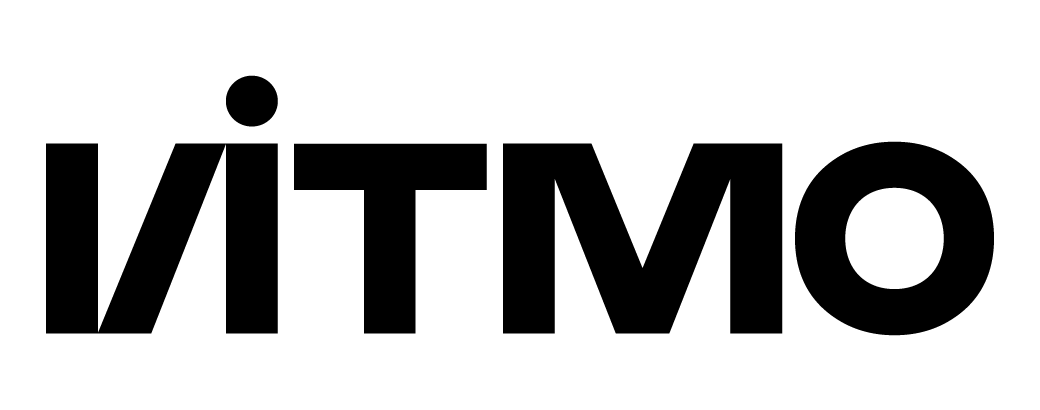
\includegraphics[scale=0.2]{../../img/itmo.png}
\end{center}
\vspace{4cm}


\begin{center}
  \large \textbf{Вариант \textnumero 16}\\
  \textbf{Лабораторная работа \textnumero 2}\\
  по дисциплине\\
  \textbf{Информатика}
\end{center}

\vspace*{\fill}

\begin{flushright}
  Выполнил Студент группы P3115\\
  \textbf{Владимир Мацюк}\\
  Преподаватель: \\
  \textbf{Малышева Татьяна Алексеевна}\\
\end{flushright}

\vspace{1cm}

\begin{center}
  г. Санкт-Петербург\\
  2022г.
\end{center}

\newpage

\lstset{
  inputencoding=utf8,
  frame=single,
  language=Java,
  breaklines=true,
  numbers=left,
  postbreak=\mbox{\textcolor{red}{$\hookrightarrow$}\space},
  extendedchars=false,
  showspaces=false,
  showstringspaces=false,
  basicstyle=\footnotesize\ttfamily,
  identifierstyle=\bf\ttfamily\color[HTML]{2a72de},
  commentstyle=\color[rgb]{0.133,0.545,0.133},
  stringstyle=\color[rgb]{0.133,0.545,0.133},
  keywordstyle=\color[HTML]{5804cf}
}

\section*{Текст задания}

\begin{enumerate}
  \item 59 0010100
  \item 51 1010011
  \item 73 0010101
  \item 95 1011110
  \item 17 011000100010001
  \item 1180
\end{enumerate}


\section*{Вывод}
Я освежил свои знания о системах счисления и выполнил переводы чисел между ними.
\end{document}
